\documentclass[aspectratio=169,14pt,usenames,dvipsnames]{beamer}
\usetheme{TalentSprint}
\usepackage[utf8]{inputenc}
\usepackage{graphics}
\usepackage{ragged2e}
\usepackage{amsfonts}
\usepackage{xcolor}
\usepackage{mathtools}
\usepackage{tcolorbox}
\usepackage{setspace}
\usepackage{lmodern}
\definecolor{swe}{rgb}{0.19, 0.73, 0.56}
\definecolor{lgreen}{RGB}{190,200,198}
\title[Perceptron, NN, and GD]{Perceptron, NN, and GD}

\begin{document}

{\1
\begin{frame} \vspace{35pt}
	\title[Perceptron]{Perceptron}
	
	\maketitle
\end{frame}
}

% Page 2
\begin{frame}{Perceptron: An Artificial Neuron}
\begin{columns}
\column{0.5\textwidth}

\begin{itemize}
  \item An artificial neuron (also referred to as a perceptron) is a mathematical function.
  \item It takes one or more inputs that are multiplied by values called “weights” and added together.
  \item A perceptron consists of: 
  	\begin{itemize}
		\item n inputs  X_{1}, X_{2}, . . . , X_{n}
		\item n weights  W_{1}, W_{2} . . . , W_{n}
		\item one output, Y  
	\end{itemize}
  \item Summed Input = \sum_{i}^{}w_{i}x_{i}
\end{itemize}
\column {0.5\textwidth}
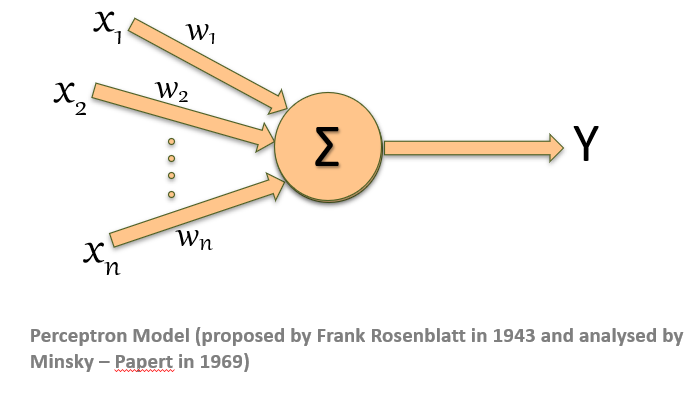
\includegraphics[width=0.8\textwidth, height=0.6\textheight]{Images/AIML_Percep_IMG1.png}
\end{columns}
\end{frame}

% Page 3
\begin{frame}{Perceptron: Biological Neuron}
\begin{columns}
\column{0.5\textwidth}

\begin{itemize}
  \item Human neural system has been a natural source of inspiration for artificial intelligence researchers. 
  \item Functioning of a neuron:  
  	\begin{itemize}
		\item dendrites receive signals
		\item cell body process them
		\item axon send signals out to other neurons
	\end{itemize}
\end{itemize}
\column {0.5\textwidth}
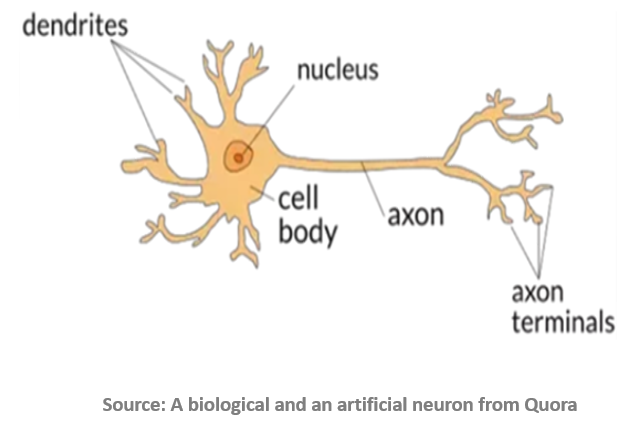
\includegraphics[width=0.8\textwidth, height=0.6\textheight]{Images/AIML_Percep_IMG2.png}
\end{columns}
\end{frame}

% Page 4
\begin{frame}{Simple Model of Neural Networks}
\begin{columns}
\column{0.5\textwidth}

\begin{itemize}
  \item Consider three inputs and one output (Y).\\ \begin{bmatrix}
 		 x_{0}\\
 		 x_{1}\\
 		 x_{2}\\
 		 x_{3}
		\end{bmatrix}
  
\end{itemize}
\column {0.5\textwidth}
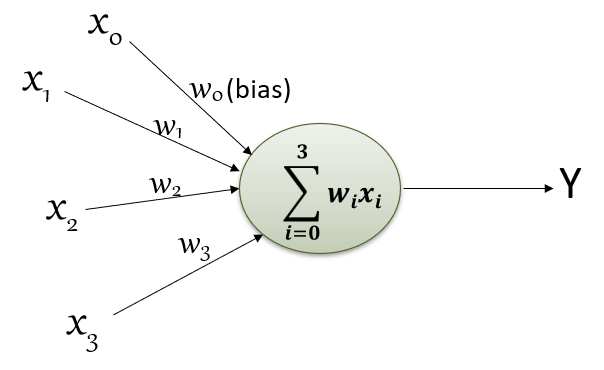
\includegraphics[width=0.8\textwidth, height=0.6\textheight]{Images/AIML_Percep_IMG3.png}
\end{columns}
\end{frame}

% Page 4
\begin{frame}{Simple Model of Neural Networks}
\begin{columns}
\column{0.5\textwidth}

\begin{itemize}
  \item Input variable’s importance is determined by the respective weights assigned to the inputs.\\
    \begin{bmatrix}
        w_{0} & w_{1} & w_{2} & w_{3} \\
    \end{bmatrix}
  
\end{itemize}
\column {0.5\textwidth}
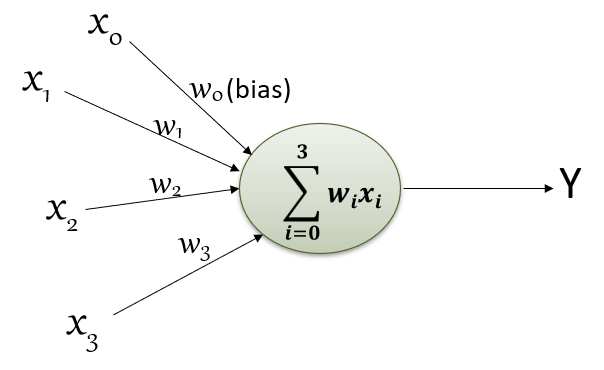
\includegraphics[width=0.8\textwidth, height=0.6\textheight]{Images/AIML_Percep_IMG3.png}
\end{columns}
\end{frame}

% Page 4
\begin{frame}{Simple Model of Neural Networks}
\begin{columns}
\column{0.5\textwidth}

\begin{itemize}  
  \item The computation inside the neuron, multiply all inputs of X by weights W and then adds them up.\\
    	
      	\begin{itemize} w_{0}x_{0} + w_{1}x_{1} + w_{2}x_{2} + w_{3}x_{3} \end{itemize}
      	\begin{itemize}= \sum_{i=0}^{3} w_{i}x_{i} \end{itemize}
     
\end{itemize}
\column {0.5\textwidth}
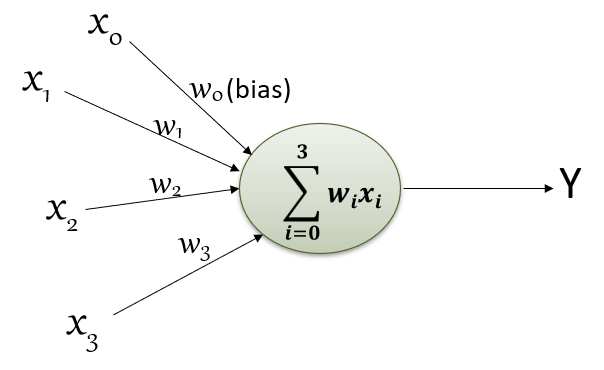
\includegraphics[width=0.8\textwidth, height=0.6\textheight]{Images/AIML_Percep_IMG3.png}
\end{columns}
\end{frame}

% Page 5
\begin{frame}{Activation Function}
\begin{itemize}
\item Activation function determines the output of the neuron based on the summed, weighted inputs. \\
\centering
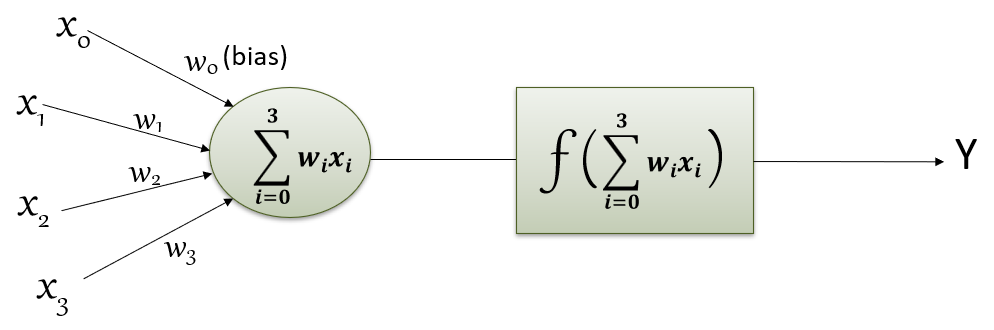
\includegraphics[width=4.5cm , height=3.5cm]{Images/AIML_Percep_IMG4.png}
\end{itemize}
\end{frame}

% Page 6
\begin{frame}{Output of Perceptron}
\begin{columns}
\column{0.5\textwidth}

\begin{itemize}
  \item If weighted sum is less than zero then the result will be 0, otherwise it will be 1. \\
    \begin{itemize}output(Y) = 1 \hspace{0.15cm} if \hspace{0.15cm} \sum_{i}^{}w_{i}x_{i}\geq 0 \end{itemize}
    \begin{itemize}or \hspace{0.15cm} 0 \hspace{0.15cm} if \hspace{0.15cm} \sum_{i}^{}w_{i}x_{i}< 0 \end{itemize}
  \item Single Perceptron can learn linearly separable patterns which gives a binary output as 1 or 0.
\end{itemize}
\column {0.5\textwidth}
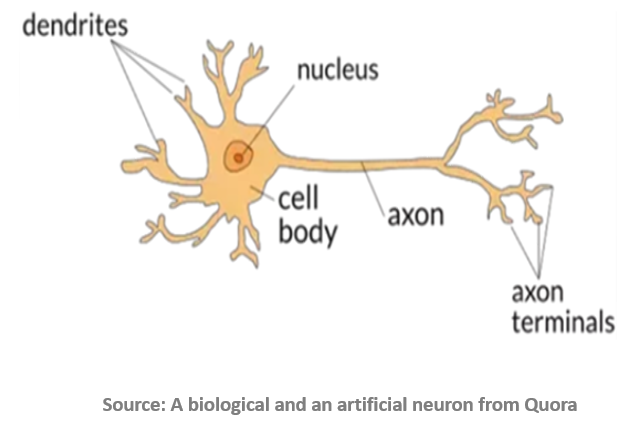
\includegraphics[width=0.8\textwidth, height=0.6\textheight]{Images/AIML_Percep_IMG2.png}
\end{columns}
\end{frame}

% Page 7
\begin{frame}{Perceptron Learning Rule}
\begin{itemize}
\item Network starts its learning by assigning a random value to each weight.
\item Calculate the output value and compare with the expected value.
\item Calculate the error – usually sum of squares of errors.
\end{itemize}
\end{frame}

% Page 7
\begin{frame}{Perceptron Learning Rule}
\begin{itemize}
\item Adjust the weights till error is minimized.
\end{itemize}
\centering
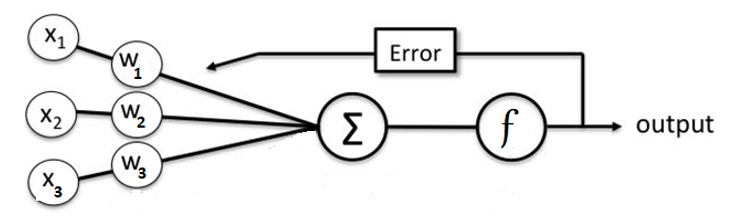
\includegraphics[width=6.5cm , height=4.0cm]{Images/AIML_Percep_IMG5.png}
\end{frame}

% Page 8
\begin{frame}{Adjusting Weights}
\begin{itemize}
\item Compare Predicted value and Actual value
\item Optimize the weights
\end{itemize}
\centering
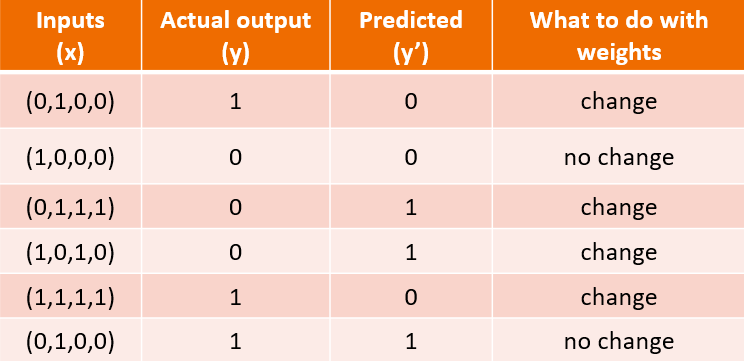
\includegraphics[width=7.5cm , height=4.0cm]{Images/AIML_Percep_IMG6.png}
\end{frame}

% Page 9
\begin{frame}{Mathematical Model}
\begin{columns}
\column{0.5\textwidth}
\item Consider one sample from Iris dataset as inputs
	\begin{itemize}
	  \item sepal length = 5.4\\
	  \item sepal width  = 3.7\\
	  \item petal length = 1.5\\
	  \item petal width = 0.2
  
\end{itemize}
\column {0.5\textwidth}
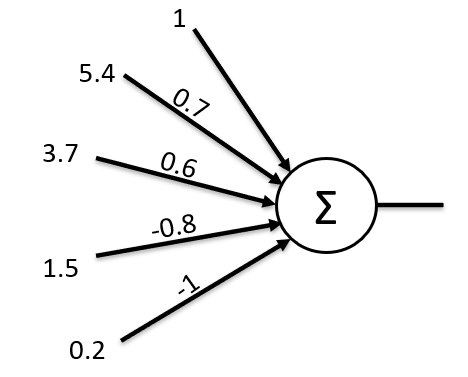
\includegraphics[width=0.8\textwidth, height=0.6\textheight]{Images/AIML_Percep_IMG7.png}
\end{columns}
\end{frame}

% Page 9
\begin{frame}{Mathematical Model}
\begin{columns}
\column{0.5\textwidth}
\item Random weights given as:
	\begin{itemize}
	  \item w1 = 0.7\\
	  \item w2 = 0.6\\
	  \item w3 = -0.8\\
	  \item w4 = -1.0  
\end{itemize}
\item Classes are Versicolor (0) or Setosa (1)
\column {0.5\textwidth}
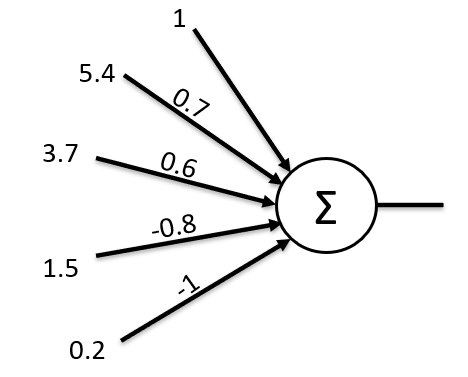
\includegraphics[width=0.8\textwidth, height=0.6\textheight]{Images/AIML_Percep_IMG7.png}
\end{columns}
\end{frame}

% Page 10
\begin{frame}{Mathematical Model}
\begin{itemize}
\item Weighted sum of the perceptron’s inputs and weights is 5.6
\item As the weighted sum is greater than zero, it gives output as 1. 
\end{itemize}
\centering
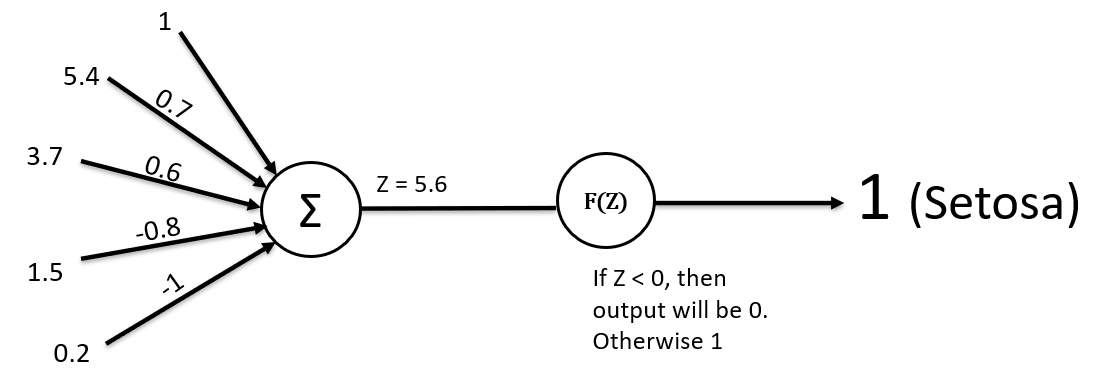
\includegraphics[width=7.5cm , height=4.0cm]{Images/AIML_Percep_IMG8.png}
\end{frame}


% Page 11
\begin{frame}{Sample Function Using A Perceptron}
\begin{columns}
\column{0.55\textwidth}
\item Problem statement 1: 
\item If either of the two inputs are HIGH, output of the Perceptron is HIGH
\begin{itemize}
  \item Set bias as -1, W1 and W2 as 1.
  \item Calculate weighted sum
  \item Apply activation function. If weighted sum is less than the\\
   value (0), then result will be 0. Otherwise, it will be 1. 
  
\end{itemize}
\column {0.55\textwidth}
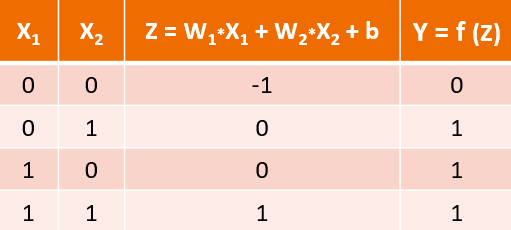
\includegraphics[width=0.6\textwidth, height=0.3\textheight]{Images/AIML_Percep_IMG9.png}
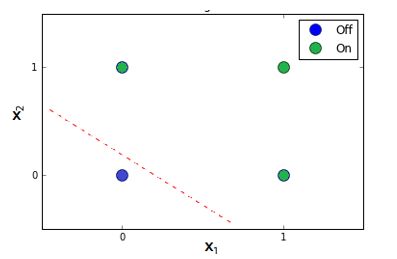
\includegraphics[width=0.6\textwidth, height=0.3\textheight]{Images/AIML_Percep_IMG10.png}
\end{columns}
\end{frame}

% Page 12
\begin{frame}{Sample Function Using A Perceptron}
\begin{columns}
\column{0.65\textwidth}
\item Problem statement 2: 
\item If both the inputs are HIGH, output of the Perceptron is HIGH.
\begin{itemize}
  \item Set bias as -1, W1 and W2 as 0.5.
  \item Calculate weighted sum
  \item Apply activation function. If weighted sum is less than the threshold\\
   value (0), then result will be 0. Otherwise, it will be 1. 
  
\end{itemize}
\column {0.65\textwidth}
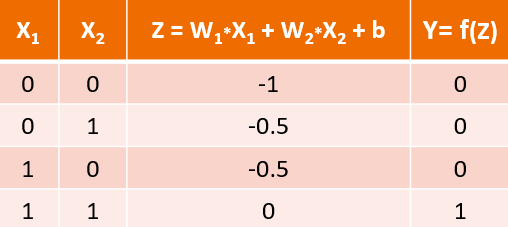
\includegraphics[width=0.5\textwidth, height=0.3\textheight]{Images/AIML_Percep_IMG11.png}
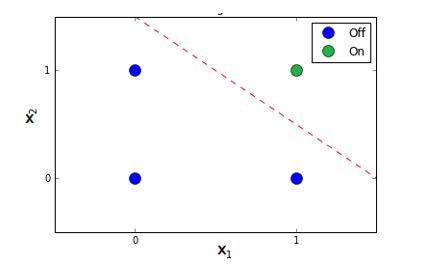
\includegraphics[width=0.5\textwidth, height=0.3\textheight]{Images/AIML_Percep_IMG12.png}
\end{columns}
\end{frame}

% Page 13
\begin{frame}{Linear Decision Boundary}
\begin{columns}
\column{0.65\textwidth}
\begin{itemize}
\item Perceptron distinguishes between the two linearly separable classes.
\item The Perceptron algorithm learns the weights in order to draw a linear decision boundary.
\end{itemize}
\column {0.65\textwidth}
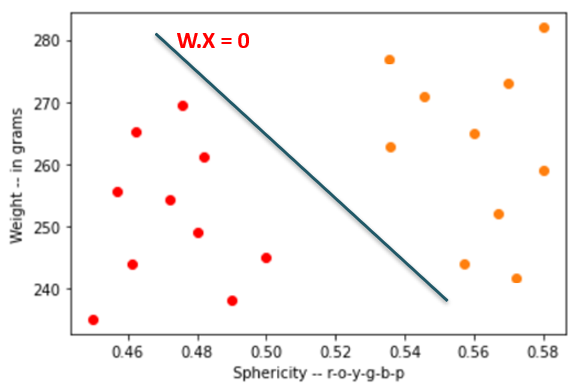
\includegraphics[width=0.5\textwidth, height=0.3\textheight]{Images/AIML_Percep_IMG13.png}
\end{columns}
\end{frame}

% Page 14
\begin{frame}{Limitations of Single Perceptron}
\begin{columns}
\column{0.65\textwidth}
\begin{itemize}
\item Perceptron can solve the problem in fig.1. It can easily separate the two classes. 
\item Perceptron cannot separate classes in fig.2
\end{itemize}
\column {0.65\textwidth}
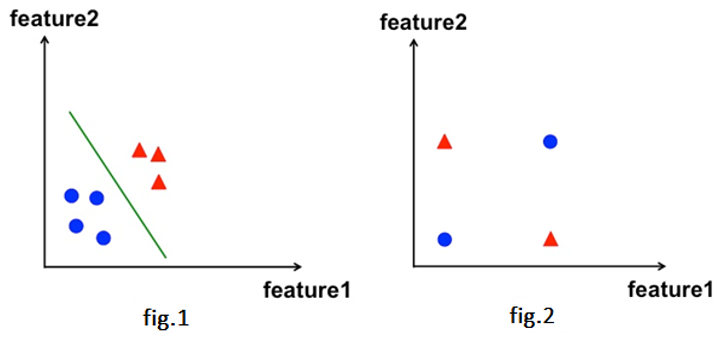
\includegraphics[width=0.5\textwidth, height=0.3\textheight]{Images/AIML_Percep_IMG14.png}
\end{columns}
\end{frame}

% Page 15
\begin{frame}{Summary}
\begin{itemize}
\item Perceptron is a two class classification algorithm in ML. 
\item Perceptron multiplies all inputs of x by weights w and then adds them up.
\item Perceptrons learn optimal weights. 
\item A single perceptron can serve as a classifier or regressor.
\end{itemize}
\centering
\end{frame}

% Page 16
{\1
\begin{frame} \vspace{35pt}
	\title[Gradient Descent ]{Gradient Descent }
	\subtitle [Introduction Lecture]{Introduction Lecture}
	
	\maketitle
\end{frame}
}

% Page 17
\begin{frame}{Gradient Descent}
\begin{itemize}
\item \textbf {Gradient} means an incline or a slope.
\item \textbf {Descent} means to move towards the bottom of the slope
\end{itemize}
\centering
\end{frame}

% Page 18
\begin{frame}{Visualizing Steepest Descent}
\centering
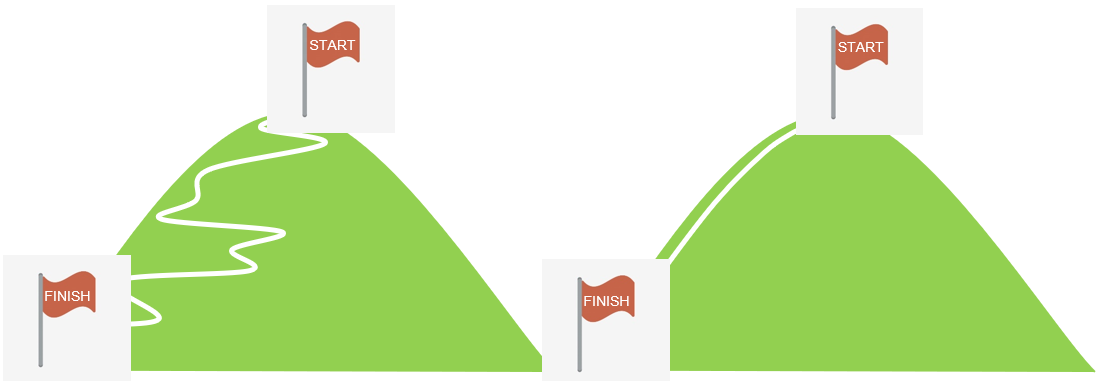
\includegraphics[width=7.5cm , height=4.0cm]{Images/AIML_Percep_IMG16.png}
\begin{itemize}
\item The most efficient way to get down, would be to follow along the steepest slope, or gradient of the hill
\end{itemize}
\end{frame}

% Page 19
\begin{frame}{Technical understanding}
\item \textbf {Objective} : Take the ball to the minimum point of the graph.
\begin{itemize}
\item Randomly select initial weight values \textbf{w} of the function.\\
	\begin {itemize}J(w) = w^2 \end{itemize}
\end{itemize}
\begin{itemize}
\item Set an initial value of w = 6
\end{itemize}

\centering
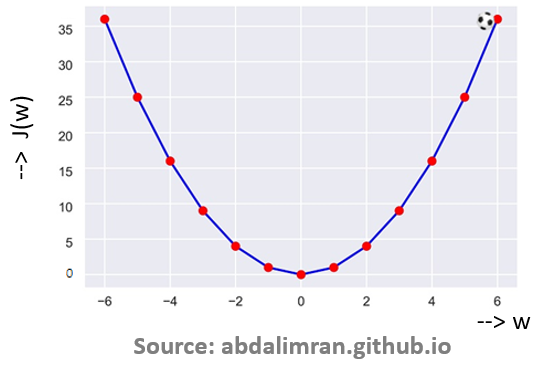
\includegraphics[width=7.5cm , height=4.0cm]{Images/AIML_Percep_IMG15.png}
\end{frame}

% Page 20
\begin{frame}{Technical understanding}
\begin{itemize}
\item To find the next position, we should know in which direction to move and how much to move.
\item Next position of w is  w' = w - \eta * J'(w) 
  \begin{itemize} 
  \item J'(w)  gives the direction of maximum increase of the function
  \item Minus of that function gives the maximum decrease of the function
  \item Step size which is measured by \eta (eta) 
  \end{itemize}  
\end{itemize}
\end{frame}

% Page 21
\begin{frame}{Methods of applying Gradient Descent}
\begin{itemize}
\item Gradient Descent can be applied at every sample
\item Gradient Descent can be applied at the end of each epoch
\item Gradient Descent can be applied after a percentage of the training samples
\end{itemize}
\end{frame}

% Page 22
\begin{frame}{Demo Experiment}
\item \textbf {Objective}: To find the minimum value of the function:
\begin{itemize}
\begin{itemize}
\hspace{1.75cm}f(x) = x^{2}+7sin(x) \hspace{0.15cm} for \hspace{0.15cm} the \hspace{0.15cm} given \hspace{0.15cm} x \hspace{0.15cm} values
\end{itemize}
\end{itemize}
\end{frame}

% Page 23
\begin{frame}{Summary}
\begin{itemize}
\item Gradient gives the direction of the function.
\item Gradient descent strategy is to move along the steepest path.
\item Gradient descent finds the minimum point of the function.
\end{itemize}
\end{frame}

% Page 24
\begin{frame}{Individual Labs}
\textbf {Perceptron Iris}
\begin{itemize}
\item The aim of this experiment is to 
\begin{itemize}
\item understand perceptron algorithm using mathematical approach (Single layer perceptron) 
\item randomly Initializing the inputs and weights and calculating the weighted sum and defining the step function for each feature and finding accuracy
\item training a perceptron classifier from sklearn package
\end{itemize}
\item The dataset used in this experiment is IRIS dataset
\end{itemize}
\end{frame}

{ \1
\begin{frame}
	\title{Thanks!!}
	\subtitle{Questions?}
	\maketitle
\end{frame}
}

\end{document}
